\documentclass{beamer}

\usepackage[utf8]{inputenc}
\usepackage[english]{babel}
\usepackage{etex}
\usepackage{graphicx}
\usepackage{color}
\usepackage{hyperref}
\usepackage{verbatim}
\usepackage{url}
\usepackage{moreverb}
\usepackage{fancyvrb}
\usepackage{natbib}
\usepackage{eulervm}
\usepackage{auto-pst-pdf}
\usepackage{pst-plot}
\usepackage{amssymb}
\usepackage{pifont}
\usepackage{algpseudocode}
\usepackage{multirow}

% Code snippets
\usepackage{minted}
\definecolor{rulecolor}{rgb}{0.80,0.80,0.80}
\definecolor{bgcolor}{rgb}{1.0,1.0,1.0}
\newminted{python}{bgcolor=bgcolor}

% Checked marks
\newcommand{\cmark}{\ding{51}}%
\newcommand{\xmark}{\ding{55}}%

% Colors
\newrgbcolor{mygreen}{.00 .5 .00}
\newcommand{\X}[1]{\textcolor{blue}{#1}}
\newcommand{\y}[1]{\textcolor{red}{#1}}
\newcommand{\model}[1]{\textcolor{mygreen}{#1}}
\newcommand{\loss}[1]{\textcolor{lightblue}{#1}}

% Beamer layout
\hypersetup{colorlinks=true, linkcolor=black, urlcolor=blue}
\usetheme{boxes}
\beamertemplatenavigationsymbolsempty
\setbeamertemplate{sections/subsections in toc}[circle]
\setbeamertemplate{footline}[frame number]
\setbeamertemplate{itemize items}[circle]
\setbeamertemplate{itemize subitem}[square]

% Front slide
\title{{\bf Supervised Learning}\\
Gaussian processes for regression}
\author{
Gilles Louppe (\href{https://twitter.com/glouppe}{@glouppe})
}
\date{October 17, 2016}

% Argmax
\DeclareMathOperator*{\argmax}{arg\,max}

\begin{document}

\begin{frame}[plain]
\titlepage
\end{frame}


\begin{frame}
    \frametitle{Problem statement}

    \begin{figure}
    \centering
    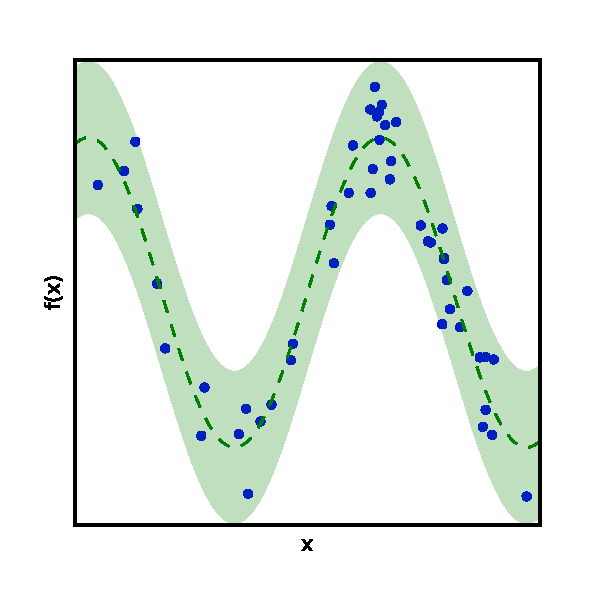
\includegraphics[width=0.65\textwidth]{./figures/regression-bars.pdf}\\
    Regression, with error bars
    \end{figure}
\end{frame}


\begin{frame}
    \frametitle{Problem statement}

    \begin{itemize}
        \item Training data ${\cal L} = \{\mathbf{x}_i, f_i\}_{i=1}^N$
        \item $\mathbf{x}_i \in \mathbb{R}^d$
        \item $y_i = f(\mathbf{x}_i)$ for some unknown $f$
        \item We wish to recover the underlying process $f$ from the observed data, i.e infer $f$ for some unseen $\mathbf{x}$, using $p(f|{\cal L})$.
    \end{itemize}
\end{frame}


\begin{frame}
    \frametitle{The multivariate gaussian distribution}

    \begin{columns}
        \begin{column}{0.6\textwidth}

        Let assume a random variable $\mathbf{f}$ following a multivariate
        Gaussian distribution, and let partition its dimensions into two
        sets $A$ and $B$:

        \begin{align*}
            &\underbrace{f_1, \dots, f_i}_{\mathbf{f}_A},\underbrace{f_{i+1}, \dots, f_N}_{\mathbf{f}_B}  \sim {\cal N}(\mu, K) \\
            &\mu = \begin{bmatrix}\mu_A\\
                                  \mu_B\end{bmatrix} \in \mathbb{R}^N\\
            &K = \begin{bmatrix}K_{AA} & K_{AB} \\
                                K_{BA} & K_{BB}\end{bmatrix} \in \mathbb{R}^{N \times N}
        \end{align*}

        \end{column}
        \begin{column}{0.4\textwidth}
            \begin{figure}
            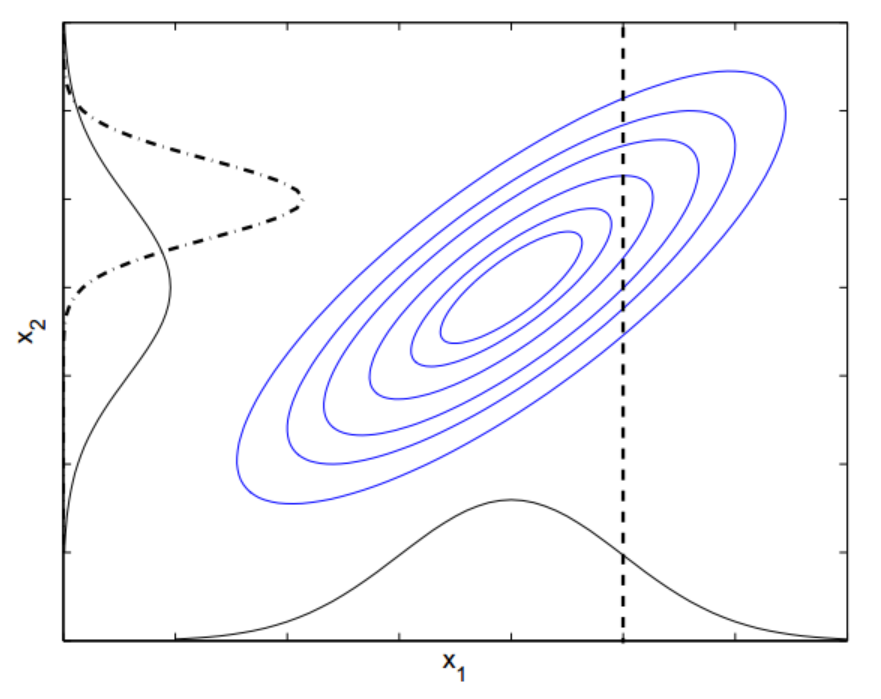
\includegraphics[width=\textwidth]{./figures/mg.png}
            \end{figure}
        \end{column}
    \end{columns}
\end{frame}


\begin{frame}
    \frametitle{Marginal and conditional distributions}

    \begin{figure}
    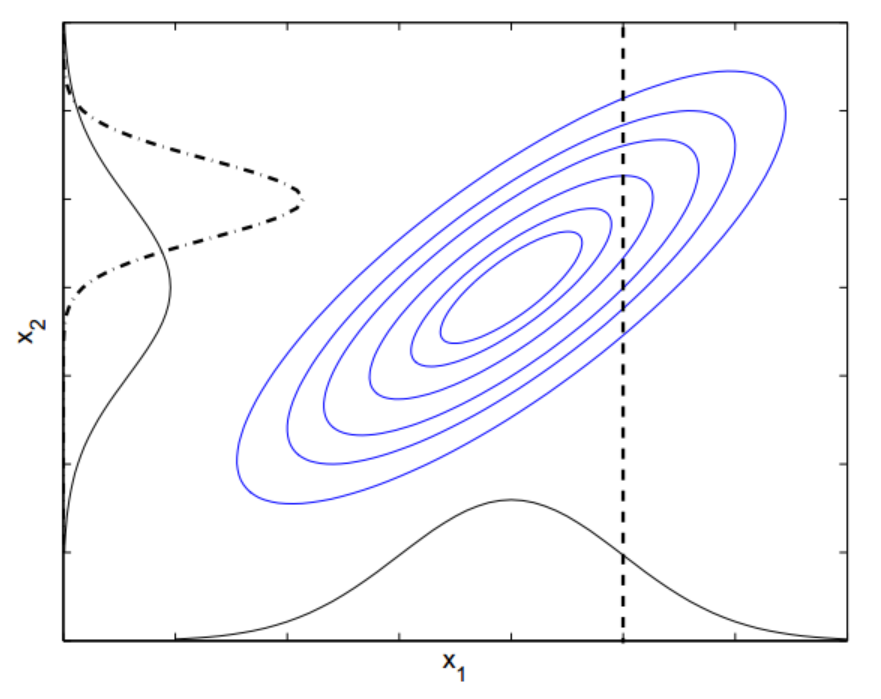
\includegraphics[width=0.4\textwidth]{./figures/mg.png}
    \end{figure}

        \begin{itemize}
            \item The {\it marginal} distribution of a multivariate gaussian is a multivariate gaussian:
            \begin{align*}
                &{\mathbf{f}_A}  \sim {\cal N}(\mu_A, K_{AA})
            \end{align*}

            \item The {\it conditional} distribution of a multivariate gaussian is a multivariate gaussian:
            \begin{align*}
                &{\mathbf{f}_A}|{\mathbf{f}_B}  \sim {\cal N}(\mu_A + K_{AB}K_{BB}^{-1}({\mathbf{f}_B} - \mu_B), K_{AA} - K_{AB}K_{BB}^{-1}K_{BA})
            \end{align*}
        \end{itemize}
\end{frame}


\begin{frame}
    \frametitle{Gaussian Processes}

    {\bf Definition.} A {\it Gaussian process} is a (potentially infinite) collection
    of random variables such that the joint distribution of any finite
    number them is multivariate Gaussian.
\end{frame}


\begin{frame}
    \frametitle{Gaussian Processes: the simpler explanation}

    \begin{center}
        A {\it Gaussian process} is a

        \vspace{1cm}

        \resizebox{\linewidth}{!}{HUGE\footnote{The dimension is the number of data points.}}

        \vspace{1cm}


        multivariate gaussian distribution.
    \end{center}
\end{frame}


\begin{frame}
    \frametitle{Gaussian distributions vs. Gaussian processes}

    \begin{columns}[t]
        \begin{column}{0.5\textwidth}
            {\bf Gaussian distribution}
            $$x \sim {\cal N}(\mu, K)$$

            \begin{itemize}
                \item Distribution over vectors.
                \item Fully specified by a mean and covariance.
                \item The position of the random variable in the vector plays the role of the index.
            \end{itemize}

        \end{column}
        \begin{column}{0.5\textwidth}
            {\bf Gaussian process}
            $$f \sim {\cal GP}(m(\cdot), k(\cdot,\cdot))$$

            \begin{itemize}
                \item Distribution over functions.
                \item Fully specified by a mean {\it function} $m$ and a covariance {\it function} $k$.
                \item The argument of the random function plays the role of the index.
            \end{itemize}

        \end{column}
    \end{columns}

\end{frame}


\begin{frame}
    \frametitle{Gaussian process prior}

    For $m(\cdot)=0$ and for any set  $A = \mathbf{x}_1, \dots,
    \mathbf{x}_M$ of test points, we may compute the covariance matrix $K_{AA}$, which defines a joint distribution $p(\mathbf{f}_A)$
    over function values at those points:
    $$\begin{bmatrix} f(\mathbf{x}_1)\\
                      \dots \\
                      f(\mathbf{x}_M) \end{bmatrix} \sim {\cal N}(\mathbf{0}, K_{AA})$$

    That is, we are marginalizing over the random variables not including in the test points.

\end{frame}

\begin{frame}
    \frametitle{Gaussian process prior}

    \begin{figure}
    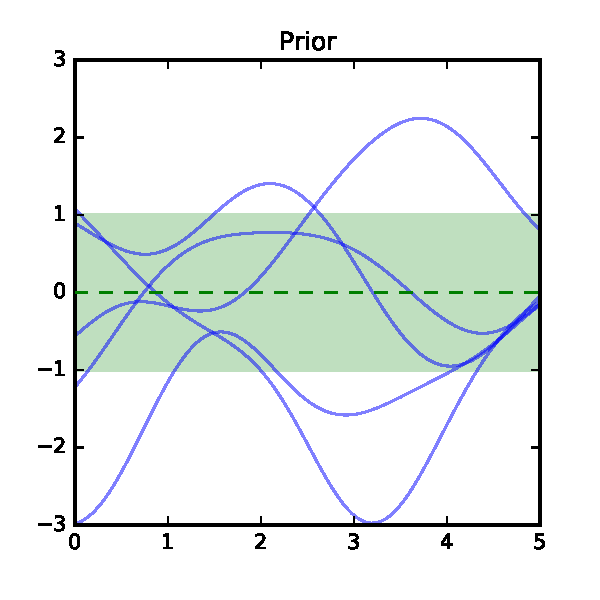
\includegraphics[width=0.8\textwidth]{./figures/gp-prior.pdf}
    \end{figure}

\end{frame}

\begin{frame}
    \frametitle{Gaussian process posterior}

    Given training data ${\cal L} = (B = \mathbf{x}_1, \dots, \mathbf{x}_N; \mathbf{f}_B = f(\mathbf{x_1}), \dots, f(\mathbf{x_N} ))$
    and test points $A = \mathbf{x}_1, \dots,
    \mathbf{x}_M$, we may similarly derive the joint distribution
    $$\begin{bmatrix}\mathbf{f}_A\\
                     \mathbf{f}_B\end{bmatrix} \sim {\cal N}(\mathbf{0}, \begin{bmatrix}K_{AA} & K_{AB} \\
                                                                                        K_{BA} & K_{BB}\end{bmatrix})$$
    on which we can condition $\mathbf{f}_B$ on the known values from ${\cal L}$,
    resulting in the posterior distribution $p(\mathbf{f}_A|{\cal L})$:

    $$\mathbf{f}_A \sim {\cal N}(K_{AB}K_{BB}^{-1}{\mathbf{f}_B}, K_{AA} - K_{AB}K_{BB}^{-1}K_{BA})$$

\end{frame}

\begin{frame}
    \frametitle{Gaussian process posterior}

    \begin{figure}
    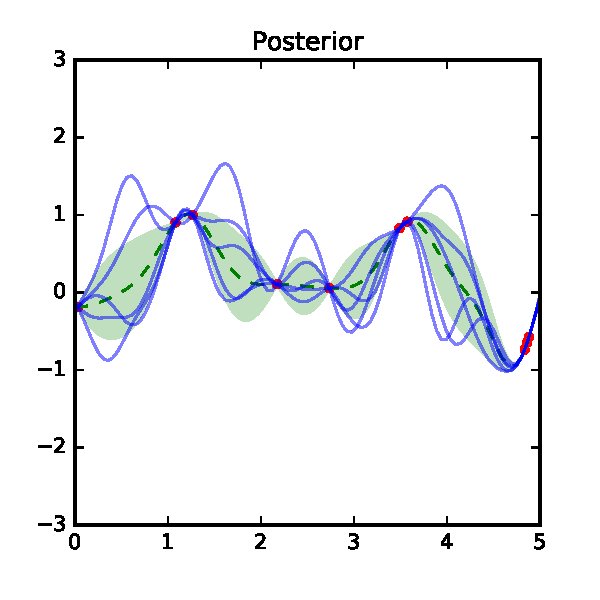
\includegraphics[width=0.8\textwidth]{./figures/gp-posterior.pdf}
    \end{figure}

\end{frame}


\begin{frame}
    \frametitle{Covariance functions (or kernels)}

    The covariance function $k(\cdot,\cdot)$ encodes the covariance between pairs of random variables $\mathbf{x}_i, \mathbf{x}_j$.
    It must be positive semi-definite and symmetric.

    \vspace{0.5cm}

    Popular examples include:
    \begin{itemize}
        \item The squared exponential function (RBF)
        \item The Matern kernel
        \item The linear kernel
        \item The polynomial kernel
        \item The white noise kernel
    \end{itemize}

    \vspace{0.5cm}

    Kernels can be composed together to describe complex interactions.
\end{frame}


\begin{frame}
    \frametitle{Squared exponential function}

    $$k(\mathbf{x}_i, \mathbf{x}_j) = \sigma^2 \exp(-  \frac{||\mathbf{x}_i - \mathbf{x}_j||^2}{2 \ell^2})$$

    Hyper-parameters:
    \begin{itemize}
        \item The length scale $\ell$ describes the smoothness of the function.
        \item The output variance $\sigma^2$ determines the average distance of the function away from its mean.
    \end{itemize}
\end{frame}


\begin{frame}
    \frametitle{Squared exponential function ($\ell=0.1$)}

    \begin{figure}
        \centering
        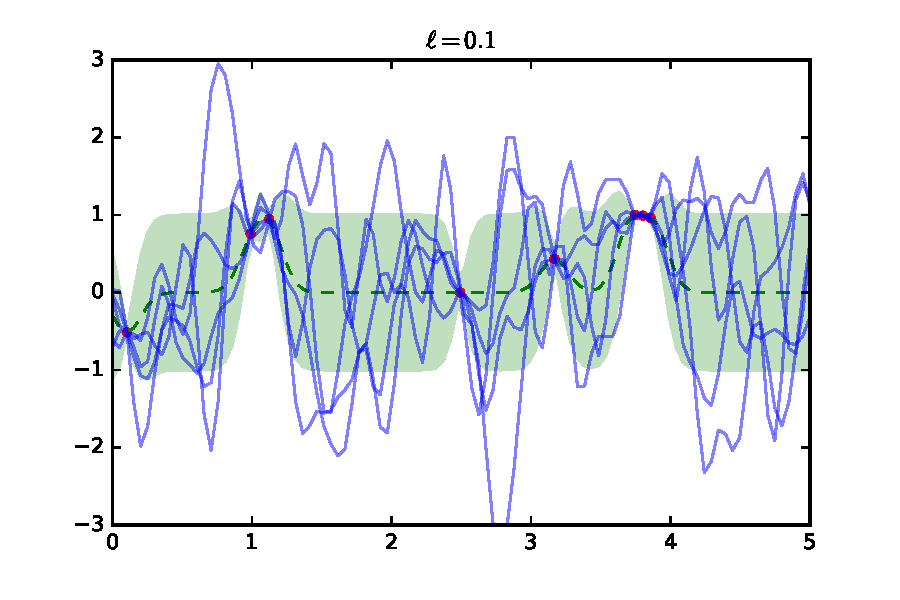
\includegraphics[width=0.8\textwidth]{./figures/rbf-01.pdf}
    \end{figure}
\end{frame}

\begin{frame}
    \frametitle{Squared exponential function ($\ell=0.5$)}

    \begin{figure}
        \centering
        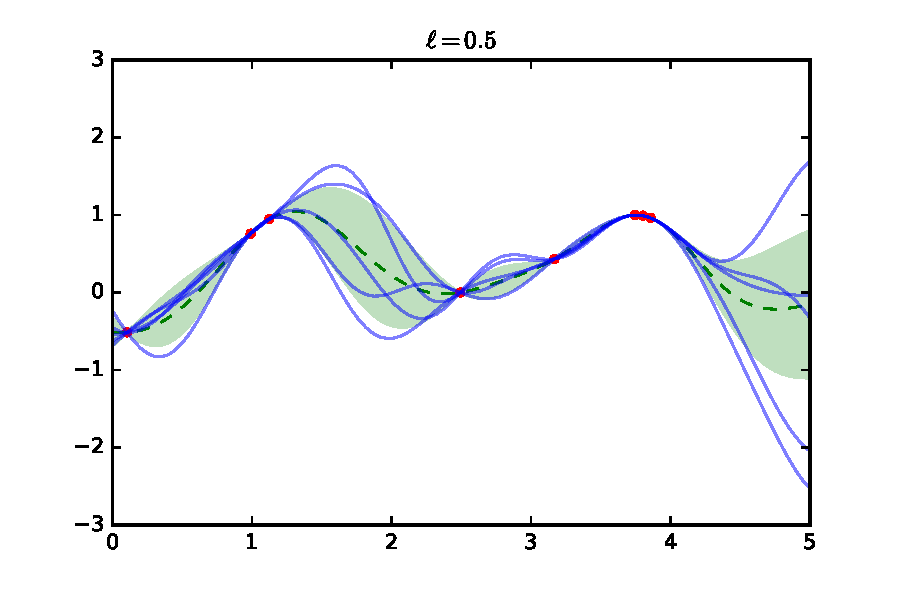
\includegraphics[width=0.8\textwidth]{./figures/rbf-05.pdf}
    \end{figure}
\end{frame}

\begin{frame}
    \frametitle{Squared exponential function ($\ell=1.0$)}

    \begin{figure}
        \centering
        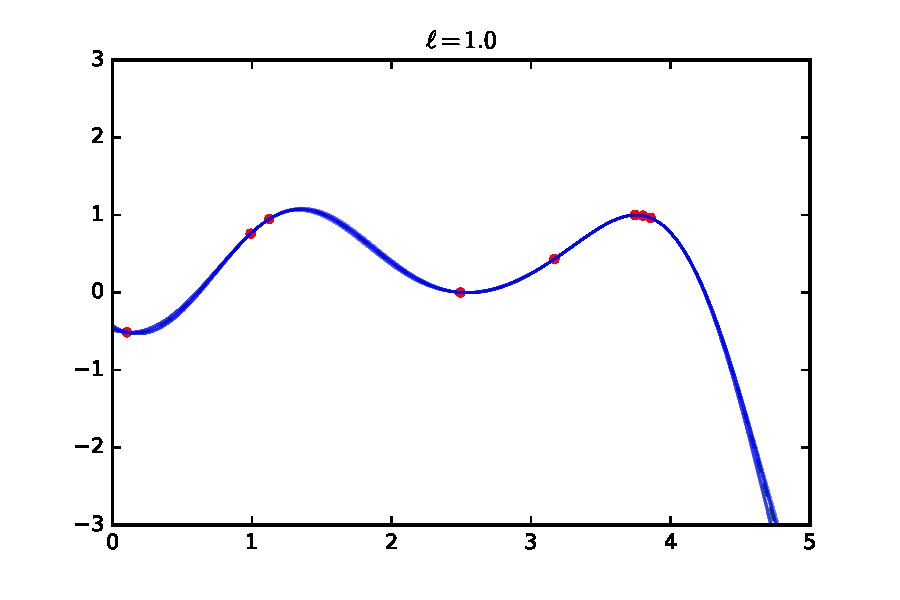
\includegraphics[width=0.8\textwidth]{./figures/rbf-10.pdf}
    \end{figure}
\end{frame}


\begin{frame}
    \frametitle{Hyper-parameters}

    \begin{itemize}
        \item So far we have assumed that the gaussian process prior $p(\mathbf{f})$
        was specified a priori.

        \item However, this distribution has itself parameters. E.g., $\ell$ and $\sigma$ when
        using the squared exponential function.

        \item Let $\theta$ denote the vector of hyper-parameters. How do we learn $\theta$?
    \end{itemize}
\end{frame}


\begin{frame}
    \frametitle{Marginal likelihood}

    Given training data ${\cal L} = (B = \mathbf{x}_1, \dots, \mathbf{x}_N; \mathbf{f}_B = f(\mathbf{x_1}), \dots, f(\mathbf{x_N} ))$,
    we can derive the prior
        $$\begin{bmatrix} f(\mathbf{x}_1)\\
                          \dots \\
                          f(\mathbf{x}_N) \end{bmatrix} \sim {\cal N}(\mathbf{0}, K_{BB;\theta})$$
    at the training points.

    Let select $\theta$ to maximize the likelihood $p(\mathbf{f}_B;\theta)$ of the training observations under that prior:
    \begin{align*}
        \theta^* &= \arg \min_\theta - \log p(\mathbf{f}_B;\theta) \\
                 &= \arg \min_\theta - \frac{1}{2} \log \det K_{BB;\theta} - \frac{1}{2} \mathbf{f}_B^T K_{BB;\theta}^{-1} \mathbf{f}_B + c
    \end{align*}

\end{frame}


\begin{frame}
    \frametitle{Squared exponential function ($\ell^*$)}

    \begin{figure}
        \centering
        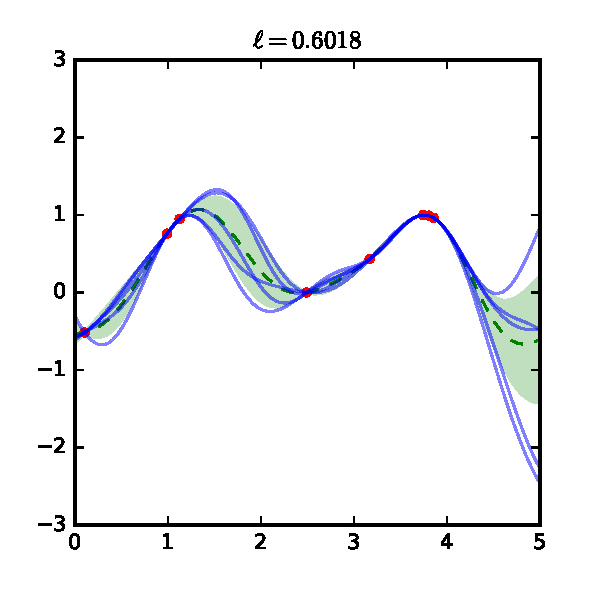
\includegraphics[width=0.8\textwidth]{./figures/rbf-ml.pdf}
    \end{figure}
\end{frame}

\begin{frame}
    \frametitle{Summary}

    \begin{itemize}
        \item Gaussians processes $=$ multivariate gaussian in infinite dimension.
        \item Provide a principled approach to derive a posterior distribution $p(\mathbf{f}|{\cal L})$.
        \item They are non-parametric, but often require a careful design of the covariance function.
        \item Gaussian processes extend to classification (not covered)
        \item They do not scale well to many observations and/or many features.
    \end{itemize}
\end{frame}


\end{document}
